%
\begin{figure}
    \centerline{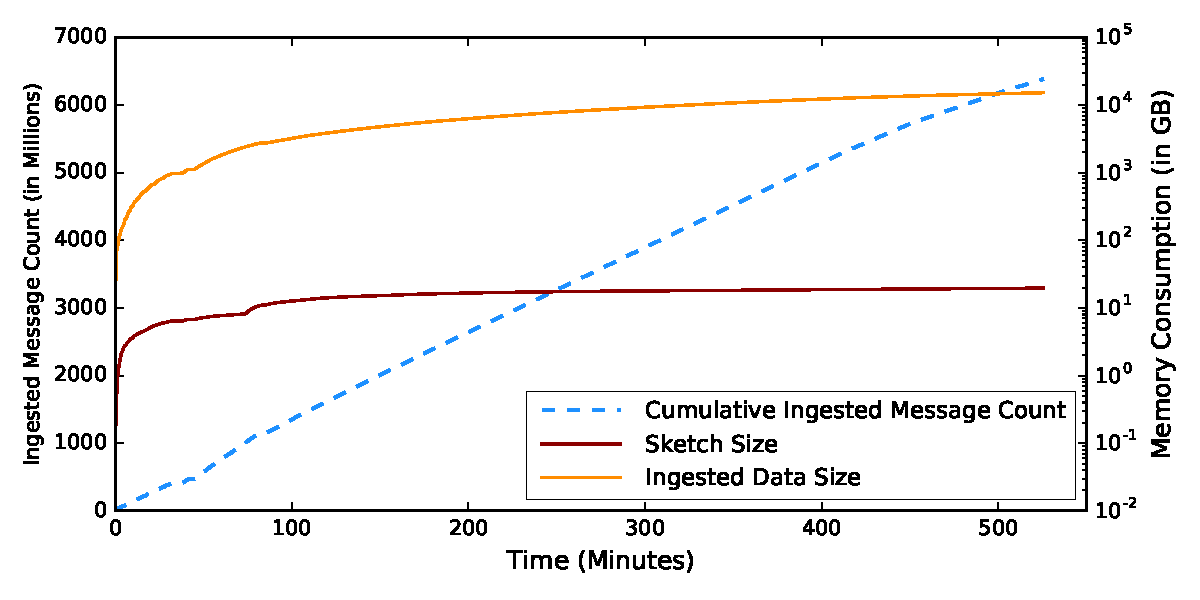
\includegraphics[width=\linewidth]{figures/ing-and-mem-usage.pdf}}
    \caption{Memory usage of the distributed sketch over time against the amount of ingested data. The rate of growth decreases over time due to the compact nature of sketchlet data structure.}
    \label{fig:dist-sketch-mem-usage}
\end{figure}
%
\section{Performance Evaluation}
Here we report system benchmarks profiling several aspects of \textsc{Synopsis}. This includes: memory consumption of the sketch, data ingestion performance of the sketch, ability to handle variable loads, organization of the sketchlets within the sketch and its query evaluation performance.
\label{sec:performance}
\subsection{Dataset and Experimental Setup}
Our subject dataset was sourced from the NOAA North American Mesoscale (NAM) Forecast System \cite{noaa_nam}.  The NAM collects atmospheric data several times per day and includes features of interest such as surface temperature, visibility, relative humidity, snow, and precipitation. Each observation in the dataset also incorporates a relevant geographical location and time of creation. This information is used during the data ingest process to partition streams across available sketchlets and preserve temporal ordering of events. The size of the entire source dataset was 25 TB.

Performance evaluations reported here were carried out on a cluster of 40 HP DL160 servers (Xeon E5620, 12 GB RAM). The test cluster was configured to run Fedora 24, and \textsc{Synopsis} was executed under the OpenJDK Java runtime 1.8.0\_72.

\subsection{Distributed Sketch Memory Evaluation}
We monitored the growth in memory consumption of the entire distributed sketch over time with continuous data ingestion as shown in Figure~\ref{fig:dist-sketch-mem-usage}. As more data was streamed into the system, the growth rate of the distributed sketch decreased as the sketchlets expanded to include vertices for their particular feature space.  At the end of our monitoring period, the total amount of ingested data was over three orders of magnitudes higher ($\sim 1285$) than the in-memory sketch size, resulting in notable space savings.
%
\subsection{Sketch Ingestion Rate}
%
\begin{table*}[bp!]
    \renewcommand{\arraystretch}{1.2}
    \caption{Profiling the update performance of sketchlet and sketch at high data ingest rates}
    \label{tab:throughput}
    \begin{center}
        \begin{tabularx}{0.9\textwidth}{|X|c|c|c|c|c|c|c|}
            \hline
            \multirow{2}{*}{Ingester Count} & \multicolumn{2}{c|}{\cellcolor[gray]{0.7}Sketchlet Throughput (msgs/s)} &\multicolumn{2}{c|}{\cellcolor[gray]{0.7}Sketch Throughput (msgs/s)} & \multicolumn{3}{c|}{\cellcolor[gray]{0.7}Sketchlet Update Latency ($\mu$s)} \\
            \cline{2-5}
             & \cellcolor[gray]{0.9}Mean & \cellcolor[gray]{0.9}Std. Dev.  &  \cellcolor[gray]{0.9}Mean & \cellcolor[gray]{0.9}Std. Dev.
             &  \cellcolor[gray]{0.9}Mean & \cellcolor[gray]{0.9}$95^{th}$ Perc. & \cellcolor[gray]{0.9}Std. Dev. \\
            \hline
            1 & 15124.562 & 575.728 & 44082.476 & 5984.503 & 64.752 & 67.175 & 5.503 \\
            \hline
            2 & 14067.452 & 491.783 & 44060.889 & 6206.208 & 64.971 & 71.170 & 4.012 \\
            \hline
            4 & 11319.321 & 1003.462 & 41645.317 & 13553.462 & 74.026 & 78.364 & 3.125 \\
            \hline
            8 & 5223.280 & 717.254 & 38369.745 & 14008.308 & 81.034 & 85.842 & 2.502 \\
            \hline
        \end{tabularx}
    \end{center}
\end{table*}
%
In this experiment, we assessed the ability of the sketch to keep pace with the high rates of incoming observational streams.
We partitioned our dataset based on timestamps of observations such that each partition comprised observations for a contiguous time period.
Within a partition, data collected in a single observation cycle for all geographical locations were stored as successive records.
Records within a single observation cycle were stored in the same order based on their locations across all observational cycles in all partitions.
Each partition was assigned a single ingester that sequentially parsed and streamed these records to the distributed sketch.
This organization of observations ensured that multiple stream ingesters target a small subset of the sketchlets to profile the \textit{worst case} performance under high stress.
This setup forces the corresponding SIFT trees to fan-out on different planes (time and features) simultaneously representing a strenuous workload on the sketch where different sections within the sketch will be stress tested over time.
A real world scenario is simulated with a single partition.

Table~\ref{tab:throughput} summarizes the results of this benchmark.
As we increase the number of ingesters with a single sketchlet, the throughput decreases due to the simultaneous fan-out operations taking place within the SIFT trees. This claim is further supported by the increase in the latency for updating the sketchlet as shown in the table.

For the sketch, we started with a single sketchlet and allowed the system to dynamically scale out and measured its throughput once it becomes stable --- when there are no frequent scaling activities.
System reached the stable state with 14-16 sketchlets in different setups.
We observed a higher throughput compared to the performance of a single sketchlet due to parallel processing of the observational stream but it did not increase linearly with the number of sketchlets.
When there is a single ingester, the throughput was constrained by the bandwidth of the machine where the ingester was running --- we were using around 86\% of the available bandwidth.
With multiple ingesters, due to the way the stream is (intentionally) constructed, the load is not evenly partitioned across the cluster --- only a subset of sketchlets were processing the stream.
%
% scale out graph
\begin{figure*}
    \centerline{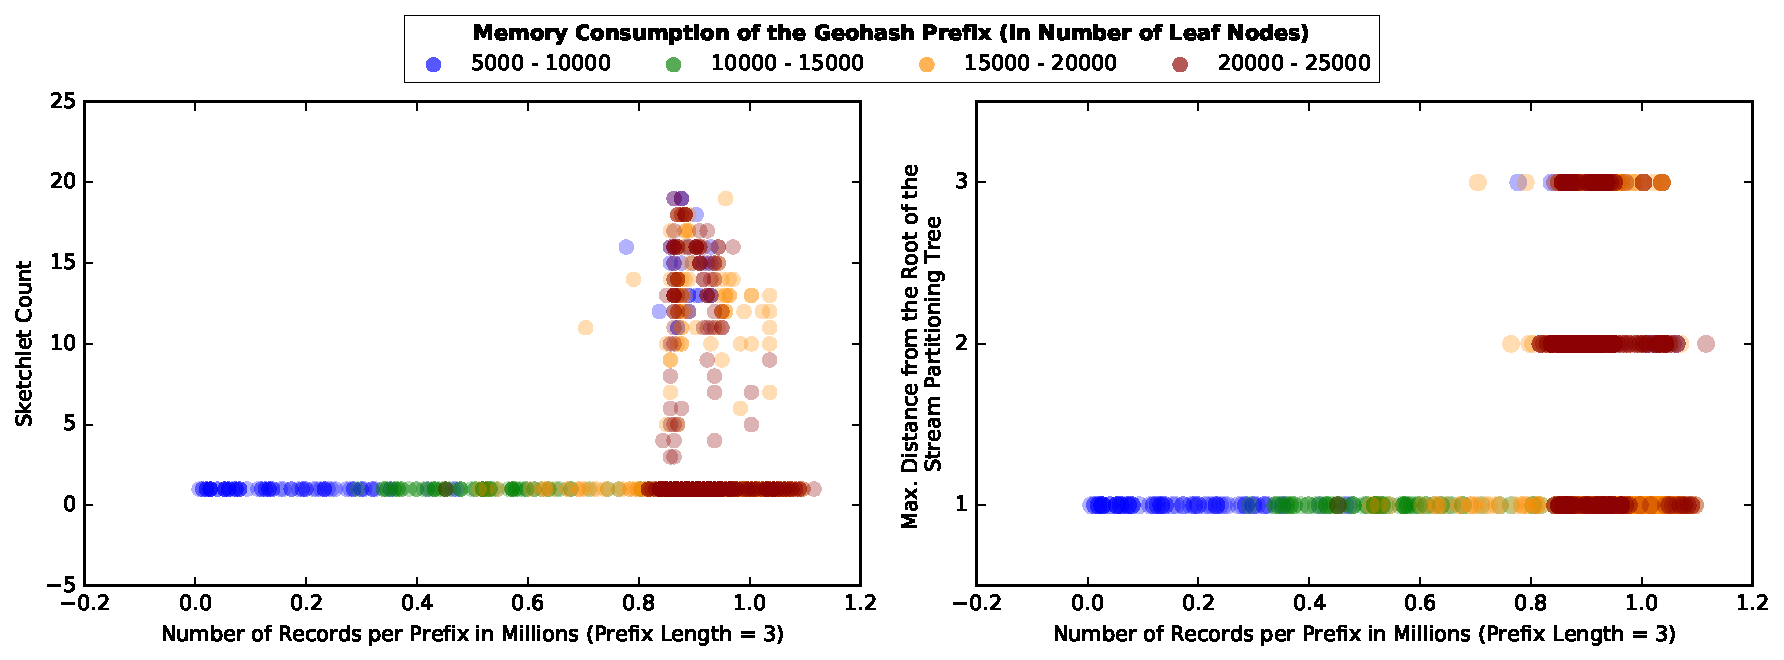
\includegraphics[width=\linewidth]{figures/scaleout_graph_analysis.pdf}}
    \caption{Analysis of a snapshot of the distributed sketch during data ingestion demonstrating the size and distribution of the information corresponding to different prefixes against the observed record count. If the information is dispersed over multiple sketchlets, it is likely to be a prefix with higher number of records and/or a wide range of observed values.}
    \label{fig:scaleout-graph-analysis}
\end{figure*}
%
\subsection{Analyzing a Snapshot of the Distributed Sketch}
Figure~\ref{fig:scaleout-graph-analysis} visualizes a snapshot of the distributed sketch which demonstrates the organization of sketchlets in runtime as described in \S\ref{sec:methodology}. 
This represents the state of the system after consuming the complete 2014 NOAA dataset and the sketch contained 48 sketchlets. 
It shows the distribution and size of the information maintained across sketchlets for each geohash prefix of length 3 characters against the number of records processed for that particular prefix.
The memory requirement for a particular geohash prefix depends on the number of records as well as the range of the observed values for different features.
The space requirement is measured by the number of leaf nodes in the corresponding sketchlets.
For the majority of the prefixes, the space requirement increases with the number of records processed.
If the data for a particular prefix is distributed across multiple sketchlets, then it is more likely to be a prefix with a high number of records as shown in the first subplot.
In such cases, some of these sketchlets are created in multiple iterations of scaling out operations from their original sketchlets which results in a higher distance from the root of the prefix tree. This is depicted in the second sub figure of Figure~\ref{fig:scaleout-graph-analysis}.
A few prefixes with high number of records can be observed with a low memory consumption and are distributed across multiple sketchlets.
Their observations spans across a smaller range, hence requires less memory but they were chosen for scaling out operations due to their high message rates. 

\subsection{Dynamic Scaling: Responding to Variable Load}
%
\begin{figure}[t!]
    \centerline{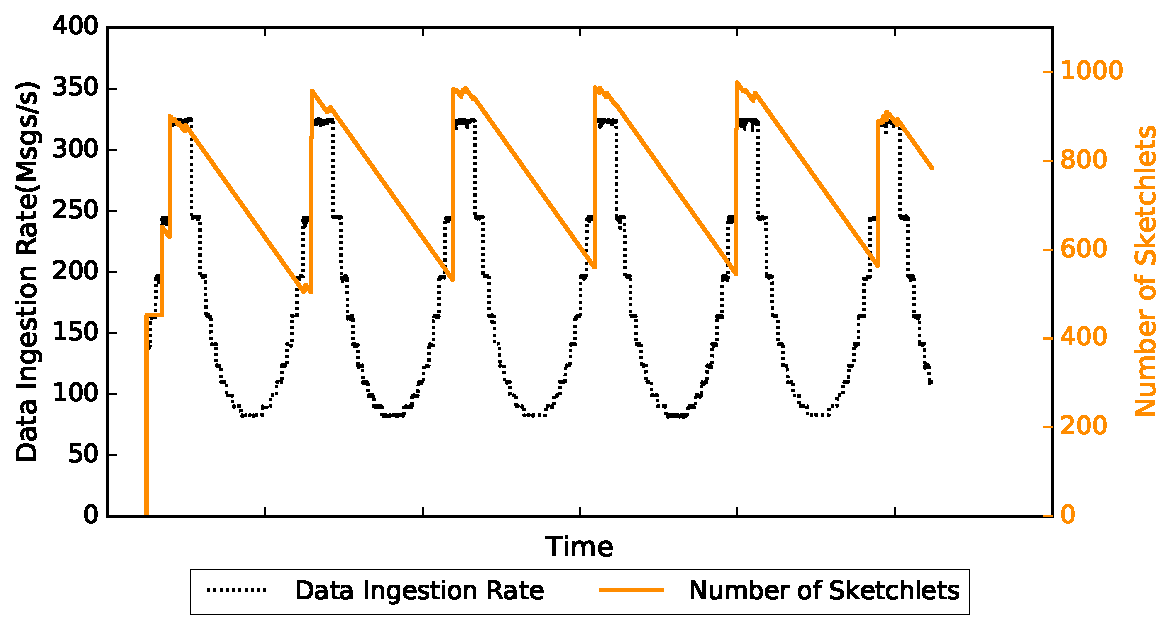
\includegraphics[width=3.5in]{figures/dyn-scaling.pdf}}
    \caption{Responding to variable load using dynamic scaling}
    \label{fig:dyn-scaling}
\end{figure}
%
We evaluated how \textsc{Synopsis} dynamically scales when the data ingestion rate is varied.
The data ingestion rate was varied over time such that the peak data ingestion rate is higher than the highest possible cumulative throughput to create a backlog at sketchlets.
We augmented the sketch update code with additional operations to match the relatively low ingestion rates used for better control.
We used the number of sketchlets within the system to quantify the scaling activities.
If the system scales out, more sketchlets will be created as a result of targeted load migration.
We started with a single sketchlet and allowed the system to dynamically scale.
As can be observed in Figure~\ref{fig:dyn-scaling}, the number of sketchlets varies with the ingestion rate.
Since we allow aggressive scale-out, rapid scaling out is observed during high data ingestion rates whereas scaling in takes place gradually with one subregion (one sketchlet) at a time.

\subsection{Query Evaluation Performance}
\begin{figure*}
    \centerline{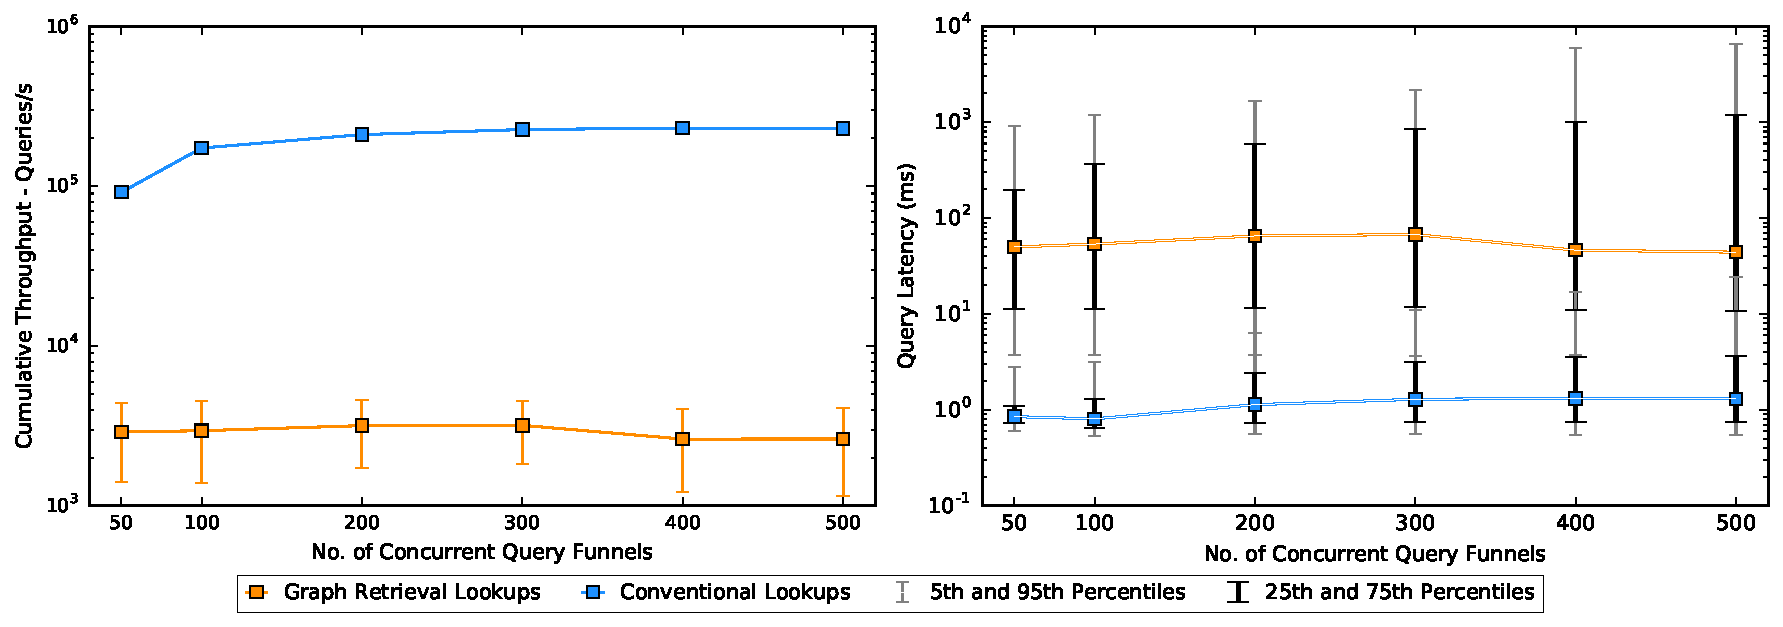
\includegraphics[width=\linewidth]{figures/query_benchmark_both.pdf}}
    \caption{Distributed query evaluation performance --- cumulative throughput and latency in a 40 node \textsc{Synopsis} cluster.}
    \label{fig:dist-query}
\end{figure*}
To evaluate distributed query performance, we executed several representative workloads across a variety of sketchlet sizes. These queries were categorized as conventional lookups and tree retrievals.  Figure~\ref{fig:dist-query} depicts the end-to-end efficiency of the query evaluations over the distributed sketch.
Cumulative query throughput and latencies were measured with varying numbers of \emph{concurrent query funnels}.
A query funnel continuously generates and dispatches random queries at its maximum possible rate to stress test the system and saturate its capacity. For example, a query could request summary statistics or feature relationships when the temperature is between 20$^{\circ}$ - 30$^{\circ}$ , humidity is above 80\%, and the wind is blowing at 16 km/h.
These randomized queries fluctuated in both the ranges of values and spatial scope, resulting in high variability in the number of sketchlets required to resolve the query as well as the depth and breadth of the required tree traversals.




